\documentclass[compress,10pt,aspectratio=169]{beamer}
\usetheme[customnumbering]{onera}

\usepackage{amsmath,amsfonts,graphicx}
\usepackage{pifont}
\usepackage{etoolbox}
\usepackage{multicol}
\usepackage{anyfontsize}
\usepackage{multirow}
\usepackage{hyperref}
\usepackage{amsmath}
\usepackage{fancybox}
\usepackage{colortbl}
\usepackage{tcolorbox}
%\setlength{\columnseprule}{1pt}
%\def\columnseprulecolor{\color{blue}}
\usepackage{minted} % syntax coloring. 
\setminted{encoding=utf-8, autogobble}
\usemintedstyle{xcode}
\AtBeginEnvironment{minted}{\fontsize{7}{7}\selectfont}

%\usepackage{dsfont}
\usepackage{ifdraft}
\ifdraft{
  \usepackage{fancyvrb}
  \DefineVerbatimEnvironment{cppcode}{Verbatim}{}
}{
\newminted{cpp}{}
}
\usepackage{hyperref}
\usetikzlibrary{shadows, arrows, decorations.pathmorphing, fadings, shapes.arrows, positioning, calc, shapes, fit, matrix,math}

\definecolor{lightblue}{RGB}{0,200,255} 
\definecolor{paper}{RGB}{255,247,197}
\definecolor{ocre}{RGB}{243,102,25} % Define the orange color used for highlighting throughout the book
\definecolor{BurntOrange}{RGB}{238,154,0}
\definecolor{darkorange}{RGB}{119, 77, 0}
\definecolor{OliveGreen}{RGB}{188,238,104}
\definecolor{DarkGreen}{RGB}{0,128,0}
\definecolor{BrickRed}{RGB}{238,44,44}
\definecolor{Tan}{RGB}{210,180,140}
\definecolor{Aquamarine}{RGB}{127,255,212}
\definecolor{NavyBlue}{RGB}{0,64,128}
\definecolor{DarkYellow}{RGB}{192,192,0}
\definecolor{Yellow}{RGB}{255,255,0}
\definecolor{navyblue}{rgb}{0.1,0.2,0.7}

\tikzset{square matrix/.style={
    matrix of nodes,
    column sep=-\pgflinewidth, row sep=-\pgflinewidth,
    nodes={draw,
      minimum height=#1,
      anchor=center,
      text width=#1,
      align=center,
      inner sep=0pt
    },
  },
  square matrix/.default=1.2cm
}

\setbeamercovered{transparent}

\title[Parallel programming\hspace{2em}]{Parallel sorting algorithms}
\subtitle{Theory and implementation}
\author[X. JUVIGNY]{Xavier JUVIGNY, SN2A, DAAA, ONERA\\ \href{mailto:xavier.juvigny@onera.fr}{\texttt{xavier.juvigny@onera.fr}} }
\date[01/08/2023]{Course Parallel Programming\\- January 8th 2023 -}
\institute{\inst{1}ONERA,\inst{2}DAAA}

\AtBeginSection[]{
  \begin{frame}{Overview}
  \begin{multicols}{2}
  \small \tableofcontents[currentsection, hideallsubsections]
  \end{multicols}
  \end{frame} 
}


\begin{document}

\MakeTitlePage

\begin{frame}
\frametitle{Table of contents}
\begin{multicols}{2}
\tableofcontents[hideallsubsections]
\end{multicols}
\end{frame}

\section{Theory of parallel sorting algorithms}

\begin{frame}[fragile]{Complexity of sorting algorithms}
  \scriptsize
  \begin{block}{Basic operations}
    \begin{itemize}
    \item \textbf{Compare algorithm} : Comparaison algorithm complexity is supposed $\mathcal{O}(1)$. But in distributed parallel context, one must consider the distribution of the initial data
      to insert the cost of data exchange between processes !
    \item  \textbf{Exchange algorithm} : Exchange algorithm complexity is supposed $\mathcal{O}(1)$. But same consideration to do as \textbf{compare algorithm};
    \item Sequential ``compare--and--exchange'' algorithm:
\begin{minted}{C++}
if (a>b) { // Comparaison
  // Exchange
  tmp = a;
  a   = b;
  b   = tmp;   }
\end{minted}
    \end{itemize}
  \end{block}
\end{frame}

\begin{frame}[fragile]{Potential speed-up}
  \scriptsize
\begin{multicols}{2}
  \begin{center}
    Data \textbf{and} processes are sorted \\

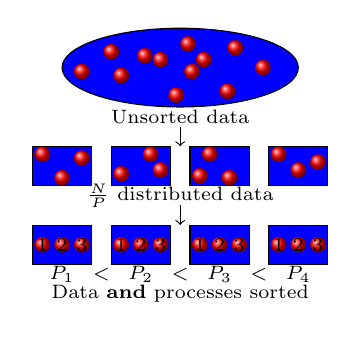
\begin{tikzpicture}[scale=0.5]
\draw[fill=blue] (0,0) ellipse (3cm and 1cm);
\shade[ball color=red] (-1.5, -0.2) circle (2mm);
\shade[ball color=red] (-0.5, 0.2) circle (2mm);
\shade[ball color=red] (-0.9, 0.3) circle (2mm);
\shade[ball color=red] (0.3, -0.1) circle (2mm);
\shade[ball color=red] (0.6, 0.2) circle (2mm);
\shade[ball color=red] (2.1, 0) circle (2mm);
\shade[ball color=red] (-2.5, -0.1) circle (2mm);
\shade[ball color=red] (-1.75, 0.4) circle (2mm);
\shade[ball color=red] (-0.1, -0.7) circle (2mm);
\shade[ball color=red] (0.2, 0.6) circle (2mm);
\shade[ball color=red] (1.4, 0.5) circle (2mm);
\shade[ball color=red] (1.2, -0.6) circle (2mm);
\draw[color=black] (0,-1.25) node {\scriptsize Unsorted data};
\draw[->] (0,-1.5) -- ( 0,-2);
\draw[fill=blue] (-3.75,-2) rectangle (-2.25,-3);
\draw[fill=blue] (-1.75,-2) rectangle (-0.25,-3);
\draw[fill=blue] (0.25,-2) rectangle (1.75,-3);
\draw[fill=blue] (2.25,-2) rectangle (3.75,-3);
\shade[ball color=red] (-3.5, -2.2) circle (2mm);
\shade[ball color=red] (-3., -2.8) circle (2mm);
\shade[ball color=red] (-2.5, -2.3) circle (2mm);
\shade[ball color=red] (-1.5, -2.7) circle (2mm);
\shade[ball color=red] (-0.75, -2.2) circle (2mm);
\shade[ball color=red] (-0.5, -2.6) circle (2mm);
\shade[ball color=red] (+0.5, -2.75) circle (2mm);
\shade[ball color=red] (+0.75, -2.2) circle (2mm);
\shade[ball color=red] (+1.25, -2.8) circle (2mm);
\shade[ball color=red] (+2.5, -2.2) circle (2mm);
\shade[ball color=red] (+3., -2.6) circle (2mm);
\shade[ball color=red] (+3.5, -2.4) circle (2mm);
\draw[color=black] (0,-3.25) node {\scriptsize$\frac{N}{P}$ distributed data };
\draw[->] (0,-3.5) -- ( 0,-4);
\draw[fill=blue] (-3.75,-4) rectangle (-2.25,-5);
\draw[fill=blue] (-1.75,-4) rectangle (-0.25,-5);
\draw[fill=blue] (0.25,-4) rectangle (1.75,-5);
\draw[fill=blue] (2.25,-4) rectangle (3.75,-5);
\shade[ball color=red] (-3.5, -4.5) circle (2mm) node {\scriptsize 1};
\shade[ball color=red] (-3., -4.5) circle (2mm) node {\scriptsize 2};
\shade[ball color=red] (-2.5, -4.5) circle (2mm) node {\scriptsize 3};
\shade[ball color=red] (-1.5, -4.5) circle (2mm) node {\scriptsize 1};
\shade[ball color=red] (-1., -4.5) circle (2mm) node {\scriptsize 2};
\shade[ball color=red] (-0.5, -4.5) circle (2mm) node {\scriptsize 3};
\shade[ball color=red] (+0.5, -4.5) circle (2mm) node {\scriptsize 1};
\shade[ball color=red] (+1., -4.5) circle (2mm) node {\scriptsize 2};
\shade[ball color=red] (+1.5, -4.5) circle (2mm) node {\scriptsize 3};
\shade[ball color=red] (+2.5, -4.5) circle (2mm) node {\scriptsize 1};
\shade[ball color=red] (+3., -4.5) circle (2mm) node {\scriptsize 2};
\shade[ball color=red] (+3.5, -4.5) circle (2mm) node {\scriptsize 3};
\draw (-3,-5.25) node {\scriptsize$P_{1}$};
\draw (-2,-5.25) node {\scriptsize$<$};
\draw (-1,-5.25) node {\scriptsize$P_{2}$};
\draw (+0,-5.25) node {\scriptsize$<$};
\draw (+1,-5.25) node {\scriptsize$P_{3}$};
\draw (+2,-5.25) node {\scriptsize$<$};
\draw (+3,-5.25) node {\scriptsize$P_{4}$};
\draw[color=black] (0,-5.75) node {\scriptsize Data \textbf{and} processes sorted};
\end{tikzpicture}
\end{center}

\begin{itemize}
\item Best sequential sorting algorithms ( for arbitrary sequences of numbers )
  have average time complexity $O(n\log n)$
\item hence, the best speedup one can except from using $n$ processors is
$
\frac{O\left(n\log n\right)}{n} = O(\log n)
$
\item there are such parallel algorithms, but the hidden constant is very large ( F. Thomson Leighton : Introduction to parallel algorithms and architectures (1991) )
\item Generally, a pratical useful $O(\log n)$ algorithm may be difficult to find.
\end{itemize}
\end{multicols}

\alert{Beware}, it may be a bad idea to take $n$ processes to sort $n$ data (granularity).
\end{frame}

\begin{frame}[fragile]{Parallelization of a naive algorithm}
  \scriptsize
  \begin{block}{Naive algorithm}
  \begin{itemize}
  \item Count the number of numbers that are smaller than a number $a$ in the list
  \item this gives the position of $a$ in the sorted list
  \item this procedure has to be repeated for all elements of the list; hence the
        time complexity is $n(n-1)=O(n^{2})$ ( not so good sequential algorithm )
  \end{itemize}
  \end{block}

  \begin{exampleblock}{Implementation}
    \begin{center}
      \shadowbox{
        \begin{minipage}{0.5\textwidth}
\begin{minted}{C++}
for ( i = 0; i < n; i++ ) {// For each value
  x = 0;
  for ( j = 0; j < n; j++ )// Computing the new pos.
    if (a[i] > a[j]) x++;
  b[x] = a[i];
}
\end{minted}
        \end{minipage}
      }
    \end{center}
  \end{exampleblock}

  Work well if there are no repetitions of the numbers in the list ( in the case
  of repetitions one has to change slightly the code ).

\end{frame}


\begin{frame}[fragile]{Rank sort : Parallel code}
  \scriptsize
  \begin{exampleblock}{Embarrasingly ``ideal'' algorithm} 
    Parallel code, using $n$ processes ( for $n$ values to sort )

    \begin{center}
      \shadowbox{
        \begin{minipage}{0.5\textwidth}
          \begin{minted}{C++}
x = 0;
for ( j = 0; j < n; j++ )
  if ( a[rank] > a[j] ) x++;
b[x] = a[rank];
          \end{minted}
        \end{minipage}
      }
    \end{center}
    \end{exampleblock}

  \begin{block}{Complexity}
    \begin{itemize}
    \item $n$ processors work in parallel to find the ranks of all numbers of the list;
    \item Parallel time complexity is $O(n)$, better than any sequential sorting algorithm !
    \item Usable for GPGPU units.
    \end{itemize}
  \end{block}
\end{frame}

\begin{frame}[fragile]{More parallelization\ldots}
  \scriptsize
  \begin{center}
    \textcolor{blue}{\bf Parallel code using $n^{2}$ processes ( for $n$ values to sort )}
  \end{center}
  \begin{block}{Parallel algorithm}
    \begin{itemize}
    \item In the case $n^{2}$ processes may be used, the comparison of each
      \texttt{a[0],\ldots,a[n-1]} with \texttt{a[i]} may be done in parallel as well
    \item Incrementing the counter is still sequential, hence the overall computation requires $1+n$ steps;
    \item If a tree structure is used to increment the counter, then the overall
      computation time is $O(\log_{2} n)$
      \begin{multicols}{2}
        
      \begin{minipage}{0.4\textwidth}
      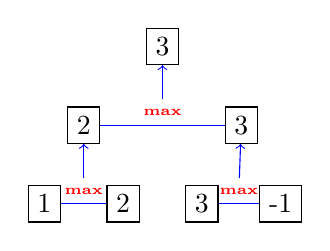
\begin{tikzpicture}
        \node[draw] (A) at (0,0)  {1};
        \node[draw] (B) at (1,0)  {2};
        \node[draw] (C) at (2,0)  {3};
        \node[draw] (D) at (3,0) {-1};

        \node[draw] (E) at (0.5,1) {2};
        \node[draw] (F) at (2.5,1) {3};
%
        \node[draw] (G) at (1.5,2) {3};
%
        \draw[blue] (A) -- (B) node[midway,above,sloped] (AB) {\tiny\textcolor{red}{\bf max}};
        \draw[blue] (C) -- (D) node[midway,above,sloped] (CD) {\tiny\textcolor{red}{\bf max}};
        \draw[blue,->] (AB) -- (E);
        \draw[blue,->] (CD) -- (F);
%
        \draw[blue] (E) -- (F) node[midway,above,sloped] (EF) {\tiny\textcolor{red}{\bf max}};
        \draw[blue,->] (EF) -- (G);
      \end{tikzpicture}
      \end{minipage}

      ( but, as one expects, processor efficiency
      is very low )\\[2mm]
      There are just theorical results : it is not efficient to use $n$ or $n^{2}$
      processors to sort $n$ numbers.
      \end{multicols}
      
      \end{itemize}
  \end{block}
\end{frame}

\begin{frame}[fragile]{Data partitionning}
  \scriptsize
  \begin{block}{\small Context}
    \begin{itemize}
    \item Usually the number $n$ of values is much larger than the number $p$ of processes;
    \item In such cases, each process will handle a part of the data (a sublist of the data)
    \end{itemize}
  \end{block}

  \begin{alertblock}{\small Distributed sorted container}
    \begin{itemize}
    \item local container is sorted;
    \item if $p_{i}<p_{j}$ then
      $\forall a_{i}\in p_{i}, \forall a_{j}\in p_{j}, a_{i} \leq a_{j}$
    \end{itemize}
  \end{alertblock}
  
  \begin{exampleblock}{\small Global scheme of parallel sort algorithm}
    For a process :
    \begin{itemize}
    \item Sort his local data;
    \item Run a merge sort algorithm to concatenate its list with that received from another process;
    \item Keep the bottom half (or the top half) of the sorted list.
    \end{itemize}
  \end{exampleblock}
\end{frame}

\begin{frame}[fragile]{Parallel compare and exchange operations}
  \scriptsize
  \begin{block}{\small Asymmetric algorithm}
    \begin{itemize}
    \item Process $p_{i}$ sends local value $A$ to process $p_{j}$;
    \item Process $p_{j}$ compares value $A$ with some local values $B_{j}$;
    \item Send the $B_{j}$ which are larger (or lesser) than $A$. If none $B_{j}$ is larger (or lesser) than $A$, sends back $A$;
    \end{itemize}
  \end{block}

  \begin{block}{\small Symmetric algorithm}
    \begin{itemize}
    \item Processes $p_{i}$ and $p_{j}$ sends some value to the other;
    \item Each process compares his value with the received value;
    \item Each process keeps his value or the received value relative to the comparaison result;
    \end{itemize}
  \end{block}

  
  \begin{alertblock}{\small Remarks}
    \begin{itemize}
    \item Data exchanges between processes is very expensive, so find some algorithms which minimize data exchanges;
    \item Generally, the receive operation doesn't know the number of values to receive $\Rightarrow$ one must probe the
          received message to get the number of data to receive, allocate the relative buffer and receive the data !
    \end{itemize}
  \end{alertblock}
\end{frame}

\begin{frame}[fragile]{Scheme of a general algorithm for parallel sort algorithm}

\begin{figure}
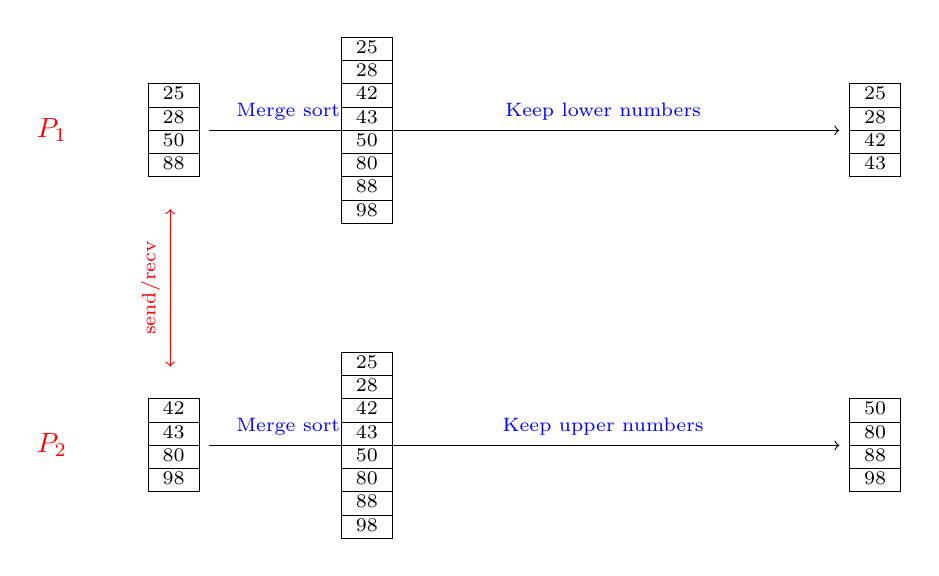
\begin{tikzpicture}
\draw node[color=red] at (-2,2) {$P_{1}$};
\draw[->] (0,2) node[left] {\scriptsize $\begin{array}{|l|}\hline
                                            25 \\ \hline
                                            28 \\ \hline
                                            50 \\ \hline
                                            88 \\ \hline \end{array}$} -- 
                                        node[above,color=blue]{\scriptsize Merge sort}
                         (2,2) node {\scriptsize $\begin{array}{|l|}\hline
                             25 \\ \hline
                             28 \\ \hline
                             42 \\ \hline
                             43 \\ \hline
                             50 \\ \hline
                             80 \\ \hline
                             88 \\ \hline
                             98 \\ \hline \end{array}$} --
                         node[above,color=blue]{\scriptsize Keep lower numbers}
                         (8,2) node[right] {\scriptsize $\begin{array}{|l|}\hline
                                            25 \\ \hline
                                            28 \\ \hline
                                            42 \\ \hline
                                            43 \\ \hline \end{array}$};
\draw node[color=red] at (-2,-2) {$P_{2}$};
\draw[->] (0,-2) node[left] {\scriptsize $\begin{array}{|l|}\hline
                                            42 \\ \hline
                                            43 \\ \hline
                                            80 \\ \hline
                                            98 \\ \hline \end{array}$} -- 
                                        node[above,color=blue]{\scriptsize Merge sort}
                                        (2,-2) node {\scriptsize $\begin{array}{|l|}\hline
                             25 \\ \hline
                             28 \\ \hline
                             42 \\ \hline
                             43 \\ \hline
                             50 \\ \hline
                             80 \\ \hline
                             88 \\ \hline
                             98 \\ \hline \end{array}$} --
                         node[above,color=blue]{\scriptsize Keep upper numbers}
                         (8,-2) node[right] {\scriptsize $\begin{array}{|l|}\hline
                                            50 \\ \hline
                                            80 \\ \hline
                                            88 \\ \hline
                                            98 \\ \hline \end{array}$};
\draw[<->,color=red] (-0.5,-1) -- node[above, rotate=90]{\scriptsize send/recv} (-0.5,1);
\end{tikzpicture}
\end{figure}
\end{frame}

\section{Parallel sort algorithms}

\begin{frame}[fragile]{Sequential bubble sort algorithm}
  \scriptsize
  \begin{multicols}{2}
  \begin{block}{Bubble sort algorithm}
    \begin{itemize}
    \item Simplest, but not so efficient sequential sorting algorithm;
    \item Compare/exchange complexity :\\
      $\displaystyle
      \sum_{i=1}^{n-1}i = \frac{n(n-1)}{2} = O(n^{2})
      $
    \end{itemize}
  \end{block}

  \begin{figure}[h]
    \includegraphics[width=0.5\linewidth]{../Images/bulles.jpg}
    \caption{Analogic bubble sort}
  \end{figure}
  \end{multicols}
  
  \begin{exampleblock}{Sequential code}
    \begin{minted}{C++}
for (int i=n-1; i>0; --i)
    for (int j=0; j<i; ++j) {
      k = j+1;
      if (a[j]>a[k]) std::swap(a[j],a[k]);
    }
    \end{minted}
  \end{exampleblock}
\end{frame}

\begin{frame}[fragile]{Odd-Even sort algorithm}
  \scriptsize
  \begin{itemize}
  \item Parallelized bubble sort
  \item Based on idea that the bodies of the main loop may be overlapped
  \end{itemize}

  \begin{exampleblock}{\small ``scalar'' Algorithm : Iteration between even and odd phase}
    \begin{itemize}
    \item Even phase\hspace*{2cm} \tikz{\node[draw,circle,inner sep=0pt] at (0,0) (A) {\scriptsize 0};\node[draw,circle,inner sep=0pt] at (1,0) (B) {\scriptsize 1};
      \node[draw,circle,inner sep=0pt] at (2,0) (C) {\scriptsize 2};\node[draw,circle,inner sep=0pt] at (3,0) (D) {\scriptsize 3};
      \draw[red,<->] (A) -- (B); \draw[red,<->] (C) -- (D);} 
      \begin{multicols}{2}
        \begin{tcolorbox}[boxsep=-1mm]
          \begin{minted}{C++}
if (rank%2==0) {
  recv(&temp, (rank+1)%nbp);
  send(&value,(rank+1)%nbp);
  if (temp < A) A = temp;   }
        \end{minted}
        \end{tcolorbox}
        
        \begin{tcolorbox}[boxsep=-1mm]
        \begin{minted}{C++}
if (rank%2==1) {
  send(&value,rank-1);
  recv(&temp, rank-1);
  if (temp > A) A = temp;   }
        \end{minted}
        \end{tcolorbox}
      \end{multicols}
    \item Odd phase\hspace*{2cm} \tikz{\node[draw,circle,inner sep=0pt] at (0,0) (A) {\scriptsize 0};\node[draw,circle,inner sep=0pt] at (1,0) (B) {\scriptsize 1};
      \node[draw,circle,inner sep=0pt] at (2,0) (C) {\scriptsize 2};\node[draw,circle,inner sep=0pt] at (3,0) (D) {\scriptsize 3};
      \draw[red,<->] (B) -- (C); \draw[red,dashed, <->] (A) -- (0,0.25) -- (3,0.25) -- (D);} 
      \begin{multicols}{2}
        \begin{tcolorbox}[boxsep=-1mm]
          \begin{minted}{C++}
if (rank%2==0) {
  recv(&temp, (rank+nbp-1)%nbp);
  send(&value,(rank+nbp-1)%nbp);
  if (temp > A) A = temp;   }
          \end{minted}
        \end{tcolorbox}

        \begin{tcolorbox}[boxsep=-1mm]
          \begin{minted}{C++}
if (rank%2==1) {
  send(&value,(rank+1)%nbp);
  recv(&temp, (rank+1)%nbp);
  if (temp < A) A = temp;   }
        \end{minted}
        \end{tcolorbox}
      \end{multicols}
    \end{itemize}
    
  \end{exampleblock}
\end{frame}

\begin{frame}[fragile]{Example of even--odd parallel bubble sort}

\alert{Example : Sorting 8 numbers on 8 processes}

{\small
\begin{tabular}{c|p{2mm}p{2mm}p{2mm}p{2mm}p{2mm}p{2mm}p{2mm}p{2mm}p{2mm}p{2mm}p{2mm}p{2mm}p{2mm}p{2mm}p{2mm}}
Step & $P_{0}$ & & $P_{1}$ & & $P_{2}$ & & $P_{3}$ & & $P_{4}$ &
     & $P_{5}$ & & $P_{6}$ & & $P_{7}$ \\ \hline
 0   & 4 & \textcolor{red}{$\leftrightarrow$} & 2 & & 7 & \textcolor{red}{$\leftrightarrow$} & 8 & 
     & 5 & \textcolor{red}{$\leftrightarrow$} & 1 & & 3 & \textcolor{red}{$\leftrightarrow$} & 6 \\
 1   & 2 & & 4 & \textcolor{red}{$\leftrightarrow$} & 7 &
     & 8 & \textcolor{red}{$\leftrightarrow$} & 1 &
     & 5 & \textcolor{red}{$\leftrightarrow$} & 3 & & 6\\
 2   & 2 & \textcolor{red}{$\leftrightarrow$} & 4 & 
     & 7 & \textcolor{red}{$\leftrightarrow$} & 1 &
     & 8 & \textcolor{red}{$\leftrightarrow$} & 3 &
     & 5 & \textcolor{red}{$\leftrightarrow$} & 6 \\
 3   & 2 & 
     & 4 & \textcolor{red}{$\leftrightarrow$} & 1 &
     & 7 & \textcolor{red}{$\leftrightarrow$} & 3 &
     & 8 & \textcolor{red}{$\leftrightarrow$} & 5 &
     & 6 \\
 4   & 2 & \textcolor{red}{$\leftrightarrow$} & 1 & 
     & 4 & \textcolor{red}{$\leftrightarrow$} & 3 &
     & 7 & \textcolor{red}{$\leftrightarrow$} & 5 &
     & 8 & \textcolor{red}{$\leftrightarrow$} & 6 \\
 5   & 1 &
     & 2 & \textcolor{red}{$\leftrightarrow$} & 3 &
     & 4 & \textcolor{red}{$\leftrightarrow$} & 5 &
     & 7 & \textcolor{red}{$\leftrightarrow$} & 6 &
     & 8 \\
 6   & 1 & \textcolor{red}{$\leftrightarrow$} & 2 &
     & 3 & \textcolor{red}{$\leftrightarrow$} & 4 &
     & 5 & \textcolor{red}{$\leftrightarrow$} & 6 &
     & 7 & \textcolor{red}{$\leftrightarrow$} & 8 \\
 7   & 1 &
     & 2 & \textcolor{red}{$\leftrightarrow$} & 3 &
     & 4 & \textcolor{red}{$\leftrightarrow$} & 5 &
     & 6 & \textcolor{red}{$\leftrightarrow$} & 7 &
     & 8
\end{tabular}
}
\end{frame}

\begin{frame}[fragile]{Odd-even parallel algorithm per block}
  \scriptsize
  \begin{multicols}{2}
  \begin{block}{\small Per block algorithm}
    \begin{itemize}
    \item Replace a value per process with a sorted \\
          set of values per process
    \item Use sort-fusion algorithm to exchange values
    \item Data comparaison complexity : \\
      $
      \frac{N}{nbp}\log_{2}\left(\frac{N}{nbp}\right) +
      (nbp-1).\frac{2N}{nbp}
      $
    \item Data communication complexity : \\
      $
      (nbp-1).\frac{2N}{nbp}
      $
    \end{itemize}
  \end{block}

  \begin{exampleblock}{\small Implementation}
    \begin{minted}{C++}
sort(values);// Quick sort of local values
for (it=0; it<nbp-1; ++it) {// Odd-even algorithm
  if (it is odd) {
    if (rank is even and rank > 0) {
      receive(buffer, rank-1); send(values, rank-1);
      values = fusionSort(buffer, values, keepMax);
    } else if (rank is odd and rank < nbp-1) {
      send(values, rank+1); recv(buffer, rank+1);
      values = fusionSort(buffer, values, keepMin);
    }
  } else if (it is even) {
    if (rank is even and rank < nbp-1) {
      recv(buffer, rank+1); send(values, rank+1);
      values = fusionSort(buffer, values, keepMin);
    } else if (rank is odd) {
      send(values, rank-1); recv(buffer, rank-1);
      values = fusionSort(buffer, values, keepMax);
    }
  }
}
    \end{minted}
  \end{exampleblock}
  \end{multicols}
\end{frame}

\begin{frame}[fragile]{Shear sort algorithm}
  \scriptsize
  \begin{center}{\small Two dimensional sorting}\end{center}

  \begin{block}{\small Basic idea}
    \begin{itemize}
    \item Look at the array as a two-dimensional array (one row per process)
    \item The goal is to sort this 2D array in snakelike style : even rows increasing, odd rows decreasing;
    \item Two phases : In \textbf{even phase}, sort per row,
      in {odd phase,}, sort per column increasing from top to bottom;
    \item After $\log_{2}(N)+1$ phases, the array is snakelike-style sorted.
    \end{itemize}
  \end{block}

  \begin{multicols}{2}
  \begin{exampleblock}{Example}
    \only<1>{
\begin{tabular}{cccc}
 4  & 14 & 8  & 2  \\
 10 & 3  & 13 & 16 \\
 7  & 15 & 1  & 5  \\
 12 & 6  & 11 & 9
\end{tabular}
{\small\color{blue} Original number}}
    \only<2>{
\begin{tabular}{cccc}
 2  & 4  & 8  & 14 \\
 16 & 13 & 10 & 3  \\
 1  & 5  & 7  & 15 \\
 12 & 11 & 9  & 6
\end{tabular}
{\small\color{blue} Phase 1 -- row sort} }
    \only<3>{
\begin{tabular}{cccc}
 1  & 4  & 7  & 3  \\
 2  & 5  & 8  & 6  \\
 12 & 11 & 9  & 14 \\
 16 & 13 & 10 & 15
\end{tabular}
{\small\color{blue} Phase 2 -- col sort} }
    \only<4>{
\begin{tabular}{cccc}
1  & 3  & 4  & 7  \\
8  & 6  & 5  & 2  \\
9  & 11 & 12 & 14 \\
16 & 15 & 13 & 10
\end{tabular}
    {\small\color{blue} Phase 3 : row sort}
    }
    \only<5>{
\begin{tabular}{cccc}
1  & 3  & 4  & 2  \\
8  & 6  & 5  & 7  \\
9  & 11 & 12 & 10 \\
16 & 15 & 13 & 14
\end{tabular}
{\small\color{blue} Phase 4 : col sort} }
    \only<6>{
\begin{tabular}{cccc}
1  & 2  & 3  & 4  \\
8  & 7  & 6  & 5  \\
9  & 10 & 11 & 12 \\
16 & 15 & 14 & 13
\end{tabular}
{\small\color{blue} Final 5 : row sort} }
  \end{exampleblock}

  \begin{alertblock}{Remarques}
\begin{itemize}
    \item Embarrassingly parallel algorithm for shared memory !
    \item But not well adapted for distributed parallel architecture as is;
    \item How change this algorithm for distributed parallel architecture ?
\end{itemize}
  \end{alertblock}
\end{multicols}
\end{frame}

\begin{frame}[fragile]{Shear sort algorithm for parallel distributed memory architecture}
    \scriptsize
    \begin{center}\textcolor{blue}{\small Implementation ideas}\end{center}
    
    \begin{itemize}
        \item Same principal as odd-even algorithm : replace a value with some sets of values $S_{i}$ (one set per process);
        \item Define a relation order : $S_{i} < S_{j}$ iff $\max({S_{i}}) < \min({S_{j}})$ (In set, values ordered as increasing order)
        \item Use odd-even algorithm to parallelize the phase of sorting per row or column;
        \item Grouping processes in new communicators per rows and per columns;
        \item Play with rank numbering to alternate between increasing order and decreasing order for rows;
    \end{itemize}

    \begin{block}{\small Processes repartition}
    \begin{multicols}{2}
    \begin{minipage}{0.5\textwidth}
        \begin{figure}
            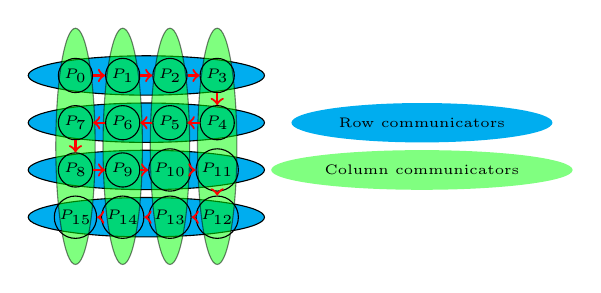
\begin{tikzpicture}
\draw[fill=cyan] (0.9, 0) ellipse  (1.5 and 0.25);
\draw[fill=cyan] (0.9, -0.6) ellipse  (1.5 and 0.25);
\draw[fill=cyan] (0.9, -1.2) ellipse  (1.5 and 0.25);
\draw[fill=cyan] (0.9, -1.8) ellipse  (1.5 and 0.25);
\draw[fill=green,opacity=0.5] (0, -0.9) ellipse  (0.25 and 1.5);
\draw[fill=green,opacity=0.5] (0.6, -0.9) ellipse  (0.25 and 1.5);
\draw[fill=green,opacity=0.5] (1.2, -0.9) ellipse  (0.25 and 1.5);
\draw[fill=green,opacity=0.5] (1.8, -0.9) ellipse  (0.25 and 1.5);
\foreach \x/\y/\r in {0/0/0, 0/1/1, 0/2/2, 0/3/3, 1/0/7, 1/1/6, 1/2/5, 1/3/4, 2/0/8, 2/1/9, 2/2/10, 2/3/11, 3/0/15, 3/1/14, 3/2/13, 3/3/12} 
{
    \node[draw, circle, inner sep=1pt] (P\r) at (0.6*\y,-0.6*\x) {\tiny $P_{\r}$};
}
\foreach \x [evaluate=\x as \y using {int(\x-1)}] in {1,...,15} {
    \draw[red, ->, thick] (P\y) -- (P\x);
}
\node[fill=cyan, ellipse] at (4.4, -0.6) {\tiny Row communicators};
\node[fill=green!50, ellipse] at (4.4, -1.2) {\tiny Column communicators};
            \end{tikzpicture}
        \end{figure}
    \end{minipage}

    \begin{minipage}{0.5\textwidth}
        \begin{itemize}
            \item Use \verb@MPI_Comm_split(comm,color,key,&newcomm)@ to define row and columns communicators;
            \item Processes calling this function with same color are inside the same new communicator;
            \item key is a value to numbering the processes inside the new communicator.
        \end{itemize}
    \end{minipage}
\end{multicols}
    \end{block}
\end{frame}

\section{Quicksort algorithm}

\begin{frame}[fragile]{Sequential quick-sort algorithm}
    \scriptsize
    \begin{block}{\small Reminder}
        \begin{itemize}
            \item Optimal sequential sorting algorithm ($\mathcal{O}(n\log_{2}(n))$) based on divide-and-conquer algorithm class;
            \item Select a number $r$ called \alert{pivot} and split the list into two sublists : one with all elements at most equal
                  to $r$, the other holding all elements greater than $r$;
            \item This procedure is recursive, applied till one element lists are obtained (which are sorted)
            \item \textcolor{DarkGreen}{\bf \underline{Example }: }
            \only<1> {
            \begin{center}
                \begin{tabular}{cccccccc}
                    4 & 2 & 7 & 8 & 5 & 1 & 3 & 6 \\
                \end{tabular}
            \end{center}
            }
            \only<2> { 
            \begin{center}
                \begin{tabular}{cccccccc}
                    4 & 2 & 7 & 8 & 5 & 1 & 3 & \textcolor{red}{6} \\
                \end{tabular}
            \end{center}
            }
            \only<3> { 
            \begin{center}
                \begin{tabular}{cccccccc}
                    4 & 2 & 5 & 1 & 3 & \textcolor{blue}{6} & 7 & 8 \\
                \end{tabular}
            \end{center}
            }
            \only<4> { 
            \begin{center}
                \begin{tabular}{cccccccc}
                    4 & 2 & 5 & 1 & \textcolor{red}{3} & \textcolor{blue}{6} & 7 & \textcolor{red}{8} \\
                \end{tabular}
            \end{center}
            }
            \only<5> { 
            \begin{center}
                \begin{tabular}{cccccccc}
                    2 & 1 & \textcolor{blue}{3} & 4 & 5 & \textcolor{blue}{6} & 7 & \textcolor{blue}{8} \\
                \end{tabular}
            \end{center}
            }
            \only<6> { 
            \begin{center}
                \begin{tabular}{cccccccc}
                    2 & \textcolor{red}{1} & \textcolor{blue}{3} & 4 & \textcolor{red}{5} & \textcolor{blue}{6} & 7 & \textcolor{blue}{8} \\
                \end{tabular}
            \end{center}
            }
            \only<7> { 
            \begin{center}
                \begin{tabular}{cccccccc}
                    \textcolor{blue}{1} & 2 & \textcolor{blue}{3} & 4 & \textcolor{blue}{5} & \textcolor{blue}{6} & 7 & \textcolor{blue}{8} \\
                \end{tabular}
            \end{center}
            }
        \end{itemize}
    \end{block}

    \begin{exampleblock}{\small Sequential code}
        \begin{minted}{C++}
            void quicksort( T* list, T* start, T* end ) {
                auto pivot = choosePivot(start,end);
                if (start < end) {
                    split(list, start, end, pivot);
                    quicksort(list, start, pivot-1);
                    quicksort(list,pivot+1, end   );
                }
            }
        \end{minted}
    \end{exampleblock}
\end{frame}

\begin{frame}[fragile]{Naive parallelization of quicksort algorithm}
    \scriptsize
    \begin{block}{Ideas}
        \begin{itemize}
            \item The class of quick-sort algortihm suggests to apply a divide-and-conquer parallelization method;
            \item The main problem of this approach is that the tree distribution ( induced by the lengths of the sublists)
                  heavily depends on pivot selection; in the worst case, the tree may consists of a single path (as a list);
            \item \textcolor{blue}{\bf Analysis} : provided an equal distribution of values within sublists is assured, one gets :
            \begin{itemize}
                \item {\scriptsize Comparaisons : $\displaystyle n + \frac{n}{2} + \frac{n}{4} + \cdots \approx 2n$}
                \item {\scriptsize Communications : $t_{s} + \frac{n}{2}t_{d} + t_{s} + \frac{n}{4}t_{d} + \cdots \approx \log_{2}(n)t_{s} + nt_{d}$ where $t_{s}$ is time to start a communication
                      and $t_{d}$ the time to transfert one element to another process.}
            \end{itemize}
            \item But only last iteration uses full parallelization !
        \end{itemize}
    \end{block}
\end{frame}

\begin{frame}[fragile]{Hyperquick sort algorithm}
    \begin{center}\textcolor{blue}{\small Binary numbering of Hypercube}\end{center}

\only<1> {
\begin{figure}[h]
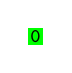
\begin{tikzpicture}[scale=1.4]
\ttfamily{}
% Cube dimension 0
\draw (-4,0) node[fill=green,inner sep=1pt]{\scriptsize 0};
\end{tikzpicture}
\caption{Dimension 0}
\end{figure}
}
%%%%%%%%%%%%%%%%%%%%%%%%%%%%%%%%%%%%%%%%%%%%%%%%%%%%%%%%%%%%%%%%%%%%%%%%%%%%%%%%%%%%%%%%%%%%%%%%%%%%%%%%%%%%%%%%%%%%%%%
\only<2> {
\begin{figure}[h]
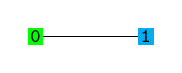
\begin{tikzpicture}[scale=1.4]
\ttfamily{}
% Cube dimension 1
\draw (-3,0) node[fill=green,inner sep=1pt](cd1_0){\scriptsize 0} -- (-2,0) node[fill=cyan,inner sep=1pt](cd1_1){\scriptsize 1};
\end{tikzpicture}
\caption{Dimension 1}
\end{figure}
}
%%%%%%%%%%%%%%%%%%%%%%%%%%%%%%%%%%%%%%%%%%%%%%%%%%%%%%%%%%%%%%%%%%%%%%%%%%%%%%%%%%%%%%%%%%%%%%%%%%%%%%%%%%%%%%%%%%%%%%%
\only<3> {
\begin{figure}[h]
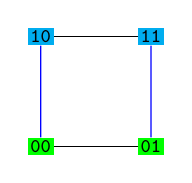
\begin{tikzpicture}[scale=1.4]
\ttfamily{}
% Cube dimension 2
\draw (-1,0) node[fill=green,inner sep=1pt](cd2_0){\scriptsize 00} -- (0,0) node[fill=green,inner sep=1pt](cd2_1){\scriptsize 01};
\draw (-1,1) node[fill=cyan,inner sep=1pt](cd2_2){\scriptsize 10} -- (0,1) node[fill=cyan,inner sep=1pt](cd2_3){\scriptsize 11};
\draw[color=blue] (cd2_0) -- (cd2_2) (cd2_1) -- (cd2_3);
\end{tikzpicture}
\caption{Dimension 2}
\end{figure}
}    
%%%%%%%%%%%%%%%%%%%%%%%%%%%%%%%%%%%%%%%%%%%%%%%%%%%%%%%%%%%%%%%%%%%%%%%%%%%%%%%%%%%%%%%%%%%%%%%%%%%%%%%%%%%%%%%%%%%%%%%
\only<4> {
\begin{figure}[h]
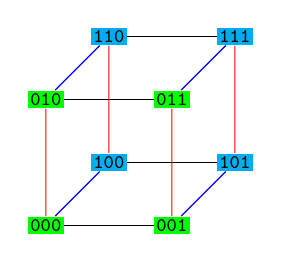
\begin{tikzpicture}[scale=1.6]
\ttfamily{}
% Cube dimension 3
\draw (1,0) node[fill=green,inner sep=1pt](cd3_0){\scriptsize 000} -- (2,0) node[fill=green,inner sep=1pt](cd3_1){\scriptsize 001};
\draw (1,1) node[fill=green,inner sep=1pt](cd3_2){\scriptsize 010} -- (2,1) node[fill=green,inner sep=1pt](cd3_3){\scriptsize 011};
\draw (1.5,0.5) node[fill=cyan,inner sep=1pt](cd3_4){\scriptsize 100} -- (2.5,0.5) node[fill=cyan,inner sep=1pt](cd3_5){\scriptsize 101};
\draw (1.5,1.5) node[fill=cyan,inner sep=1pt](cd3_6){\scriptsize 110} -- (2.5,1.5) node[fill=cyan,inner sep=1pt](cd3_7){\scriptsize 111};
\draw[color=red] (cd3_0) -- (cd3_2) (cd3_1) -- (cd3_3);
\draw[color=red] (cd3_4) -- (cd3_6) (cd3_5) -- (cd3_7);
\draw[color=blue] (cd3_0) -- (cd3_4) (cd3_1) -- (cd3_5) (cd3_2)--(cd3_6) (cd3_3)--(cd3_7);
\end{tikzpicture}
\caption{Dimension 3}
\end{figure}
}    
%%%%%%%%%%%%%%%%%%%%%%%%%%%%%%%%%%%%%%%%%%%%%%%%%%%%%%%%%%%%%%%%%%%%%%%%%%%%%%%%%%%%%%%%%%%%%%%%%%%%%%%%%%%%%%%%%%%%%%%
\only<5> {
\begin{figure}[h]
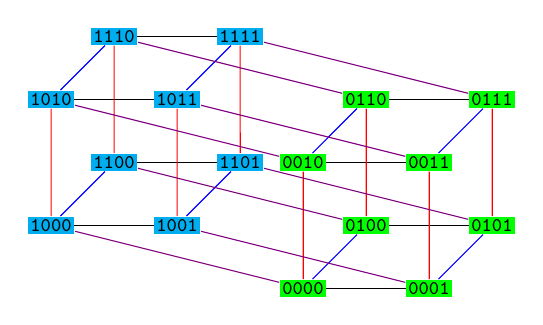
\begin{tikzpicture}[scale=1.6]
\ttfamily{}
% Cube de dimension 4
\draw (6,0) node[fill=green,inner sep=1pt](cd4_0){\scriptsize 0000} -- (7,0) node[fill=green,inner sep=1pt](cd4_1){\scriptsize 0001};
\draw (6,1) node[fill=green,inner sep=1pt](cd4_2){\scriptsize 0010} -- (7,1) node[fill=green,inner sep=1pt](cd4_3){\scriptsize 0011};
\draw (6.5,0.5) node[fill=green,inner sep=1pt](cd4_4){\scriptsize 0100} -- (7.5,0.5) node[fill=green,inner sep=1pt](cd4_5){\scriptsize 0101};
\draw (6.5,1.5) node[fill=green,inner sep=1pt](cd4_6){\scriptsize 0110} -- (7.5,1.5) node[fill=green,inner sep=1pt](cd4_7){\scriptsize 0111};
\draw[color=red] (cd4_0) -- (cd4_2) (cd4_1) -- (cd4_3);
\draw[color=red] (cd4_4) -- (cd4_6) (cd4_5) -- (cd4_7);
\draw[color=blue] (cd4_0) -- (cd4_4) (cd4_1) -- (cd4_5) (cd4_2)--(cd4_6) (cd4_3)--(cd4_7);
\draw (4,0.5) node[fill=cyan,inner sep=1pt](cd4_8){\scriptsize 1000} -- (5,0.5) node[fill=cyan,inner sep=1pt](cd4_9){\scriptsize 1001};
\draw (4,1.5) node[fill=cyan,inner sep=1pt](cd4_10){\scriptsize 1010} -- (5,1.5) node[fill=cyan,inner sep=1pt](cd4_11){\scriptsize 1011};
\draw (4.5,1) node[fill=cyan,inner sep=1pt](cd4_12){\scriptsize 1100} -- (5.5,1) node[fill=cyan,inner sep=1pt](cd4_13){\scriptsize 1101};
\draw (4.5,2) node[fill=cyan,inner sep=1pt](cd4_14){\scriptsize 1110} -- (5.5,2) node[fill=cyan,inner sep=1pt](cd4_15){\scriptsize 1111};
\draw[color=red] (cd4_8) -- (cd4_10) (cd4_9) -- (cd4_11);
\draw[color=red] (cd4_12) -- (cd4_14) (cd4_13) -- (cd4_15);
\draw[color=blue] (cd4_8) -- (cd4_12) (cd4_9) -- (cd4_13) (cd4_10)--(cd4_14) (cd4_11)--(cd4_15);
\draw[color=violet] (cd4_0) -- (cd4_8) (cd4_1) -- (cd4_9) (cd4_2) -- (cd4_10) (cd4_3) -- (cd4_11) (cd4_4) -- (cd4_12) (cd4_5) -- (cd4_13) (cd4_6) -- (cd4_14) (cd4_7) -- (cd4_15);
\end{tikzpicture}
\caption{Dimension 4}
\end{figure}
}        
\end{frame}

\begin{frame}[fragile]{Hyper quick sort algorithm (2)}
\scriptsize

\begin{block}{\small Numbering vertices of hyper-cube}
\begin{itemize}
    \item The binary numbers of two linked nodes have a difference of one bit;
    \item The distance between two nodes in a hypercube ( minimal number of nodes to access to go from
          first node to second node ) is the number of bit which differe in their binary number;
    \item It's the \textbf{Gray code} numbering.
\end{itemize}        
\end{block}

\begin{exampleblock}{\small Ideas of the hyper quick sort algorithm}
    \begin{itemize}
        \item Initially, Data are distributed across all processes;
        \item Each process sorts its local data;
        \item Loop on dimension of the hypercube and for dimension $d$, consider pair of processes $\left(p;p+2^{d}\right)$
        \item Process $p$ choose his median value as pivot and send value lesser than pivot to process $p+2^{d}$;
        \item Process $p+2^{d}$ receive pivot and data from process $p$ and keep value greater than pivot;
        \item Each process keep sorted value, using fusion sort algorithm to keep sorting.
    \end{itemize}
\end{exampleblock}
\end{frame}

\begin{frame}[fragile]{Illustration of hyper quick sort}
  
    \begin{columns}
      \column{1.5cm}
      \textbf{\scriptsize Phase 1} :
      \column{4cm}
      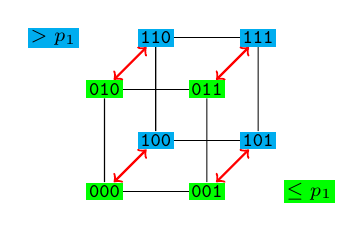
\begin{tikzpicture}[scale=1.3]
        \ttfamily{}
        % Cube dimension 3
        \draw (1,0) node[fill=green,inner sep=1pt](cd3_0){\scriptsize 000} -- (2,0) node[fill=green,inner sep=1pt](cd3_1){\scriptsize 001};
        \draw (1,1) node[fill=green,inner sep=1pt](cd3_2){\scriptsize 010} -- (2,1) node[fill=green,inner sep=1pt](cd3_3){\scriptsize 011};
        \draw (1.5,0.5) node[fill=cyan,inner sep=1pt](cd3_4){\scriptsize 100} -- (2.5,0.5) node[fill=cyan,inner sep=1pt](cd3_5){\scriptsize 101};
        \draw (1.5,1.5) node[fill=cyan,inner sep=1pt](cd3_6){\scriptsize 110} -- (2.5,1.5) node[fill=cyan,inner sep=1pt](cd3_7){\scriptsize 111};
        \draw (cd3_0) -- (cd3_2) (cd3_1) -- (cd3_3);
        \draw (cd3_4) -- (cd3_6) (cd3_5) -- (cd3_7);
        \draw[color=red,<->,thick] (cd3_0) -- (cd3_4);
        \draw[color=red,<->,thick] (cd3_1) -- (cd3_5);
        \draw[color=red,<->,thick] (cd3_2)--(cd3_6);
        \draw[color=red,<->,thick] (cd3_3)--(cd3_7);
        \draw (3,0) node[fill=green,inner sep=1pt] {\scriptsize $\leq p_{1}$};
        \draw (0.5,1.5) node[fill=cyan,inner sep=1pt] {\scriptsize $> p_{1}$};
      \end{tikzpicture}
  
      \column{1.5cm}
      \textbf{\scriptsize Phase 2} :
      \column{4cm}
      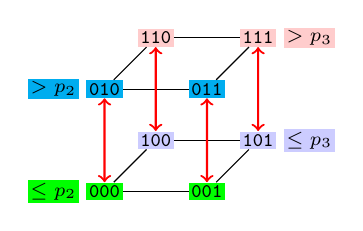
\begin{tikzpicture}[scale=1.3]
        \ttfamily{}
        % Cube dimension 3
        \draw (1,0) node[fill=green,inner sep=1pt](cd3_0){\scriptsize 000} -- (2,0) node[fill=green,inner sep=1pt](cd3_1){\scriptsize 001};
        \draw (1,1) node[fill=cyan,inner sep=1pt](cd3_2){\scriptsize 010} -- (2,1) node[fill=cyan,inner sep=1pt](cd3_3){\scriptsize 011};
        \draw (1.5,0.5) node[fill=blue!20,inner sep=1pt](cd3_4){\scriptsize 100} -- (2.5,0.5) node[fill=blue!20,inner sep=1pt](cd3_5){\scriptsize 101};
        \draw (1.5,1.5) node[fill=red!20,inner sep=1pt](cd3_6){\scriptsize 110} -- (2.5,1.5) node[fill=red!20,inner sep=1pt](cd3_7){\scriptsize 111};
        \draw[color=red,<->,thick] (cd3_0) -- (cd3_2);
        \draw[color=red,<->,thick] (cd3_1) -- (cd3_3);
        \draw[color=red,<->,thick] (cd3_4) -- (cd3_6);
        \draw[color=red,<->,thick] (cd3_5) -- (cd3_7);
        \draw (cd3_0) -- (cd3_4) (cd3_1) -- (cd3_5) (cd3_2)--(cd3_6) (cd3_3)--(cd3_7);
        \draw (0.5,0) node[fill=green,inner sep=1pt] {\scriptsize $\leq p_{2}$};
        \draw (0.5,1) node[fill=cyan,inner sep=1pt] {\scriptsize $> p_{2}$};
        \draw (3,0.5) node[fill=blue!20,inner sep=1pt] {\scriptsize $\leq p_{3}$};
        \draw (3,1.5) node[fill=red!20,inner sep=1pt] {\scriptsize $> p_{3}$};
      \end{tikzpicture}
    \end{columns}
    \vspace*{5mm}
    \begin{columns}
      \column{1.5cm}
      \textbf{\scriptsize Phase 3} :
      \column{6cm}
      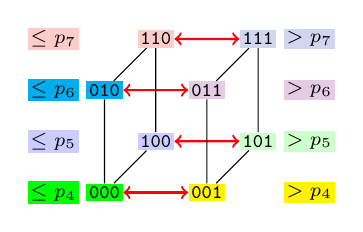
\begin{tikzpicture}[scale=1.3]
        \ttfamily{}
        \draw[color=black] (1,0) node[fill=green,inner sep=1pt] (cd3_0){\scriptsize 000};
        \draw[color=black] (2,0) node[fill=yellow,inner sep=1pt](cd3_1){\scriptsize 001};
        \draw[color=black] (1,1) node[fill=cyan,inner sep=1pt](cd3_2){\scriptsize 010};
        \draw[color=black] (2,1) node[fill=violet!20,inner sep=1pt](cd3_3){\scriptsize 011};
        \draw[color=black] (1.5,0.5) node[fill=blue!20,inner sep=1pt](cd3_4){\scriptsize 100};
        \draw[color=black] (2.5,0.5) node[fill=green!20,inner sep=1pt](cd3_5){\scriptsize 101};
        \draw[color=black] (1.5,1.5) node[fill=red!20,inner sep=1pt](cd3_6){\scriptsize 110};
        \draw[color=black] (2.5,1.5) node[fill=navyblue!20,inner sep=1pt](cd3_7){\scriptsize 111};
        % Cube dimension 3
        \draw[color=red,<->,thick] (cd3_0) -- (cd3_1);
        \draw[color=red,<->,thick] (cd3_2) -- (cd3_3);
        \draw[color=red,<->,thick] (cd3_4) -- (cd3_5);
        \draw[color=red,<->,thick] (cd3_6) -- (cd3_7);
        \draw (cd3_0) -- (cd3_2) (cd3_1) -- (cd3_3);
        \draw (cd3_4) -- (cd3_6) (cd3_5) -- (cd3_7);
        \draw (cd3_0) -- (cd3_4) (cd3_1) -- (cd3_5) (cd3_2)--(cd3_6) (cd3_3)--(cd3_7);
        \draw (0.5,0) node[fill=green,inner sep=1pt] {\scriptsize $\leq p_{4}$};
        \draw (0.5,1) node[fill=cyan,inner sep=1pt] {\scriptsize $\leq p_{6}$};
        \draw (0.5,1.5) node[fill=red!20,inner sep=1pt] {\scriptsize $\leq p_{7}$};
        \draw (0.5,0.5) node[fill=blue!20,inner sep=1pt] {\scriptsize $\leq p_{5}$};
        \draw (3,0) node[fill=yellow,inner sep=1pt] {\scriptsize $> p_{4}$};
        \draw (3,1) node[fill=violet!20,inner sep=1pt] {\scriptsize $> p_{6}$};
        \draw (3,1.5) node[fill=navyblue!20,inner sep=1pt] {\scriptsize $> p_{7}$};
        \draw (3,0.5) node[fill=green!20,inner sep=1pt] {\scriptsize $> p_{5}$};
      \end{tikzpicture}
    \end{columns}
\end{frame}

\begin{frame}[fragile]{Hyperquicksort : complexity analysis}
    \scriptsize
    \begin{itemize}
        \item Suppose we run algorithm on $nbp=2^{d}$ processes (hypercube dimension $d$);
        \item Each process holds initially $Nl=\frac{N}{nbp}$ values;
        \item \textbf{Initial sorting : } $Nl.\log_{2}(Nl)$ comparaisons;
        \item \textbf{Pivot selection : } $\mathcal{O}(1)$ (one takes middle list element) for each dimension;
        \item \textbf{Pivot broadcasting : }
        \begin{itemize}
            \item {\scriptsize Broadcast one pivot in a $k$ hypercube :  $k(t_{s}+t_{d})$;}
            \item {\scriptsize For all iterations : $(d+\cdots+1)(t_{s}+t_{d}) = \frac{d(d-1)}{2}(t_{s}+t_{d})$ compaisons;}
        \end{itemize}
        \item \textbf{Split list from pivot value : } For sorted list of size $x$, $\log_{2}(x)$ comparaisons;
        \item \textbf{Exchange part of list : } To exchange $\frac{x}{2}$ data : $2(t_{s}+\frac{x}{2}t_{d})$
        \item \textbf{Fusion merge sort : } $\frac{x}{2}$ comparaisons
    \end{itemize}

    \begin{alertblock}{\small Total (for ideal balance)}
        \begin{itemize}
            \item $N_{l}.\log_{2}(N_{l})+\left(\log_{2}(N_{l}) + \frac{N_{l}}{2}\right).d$ comparaisons
            \item $\left(\frac{d(d-1)}{2}+2d\right)t_{s} + \left(\frac{d(d-1)}{2}+d.N_{l}\right).t_{d}$ for message;
        \end{itemize}
    \end{alertblock}
\end{frame}

\section{Bitonic sorting algorithm}

\begin{frame}[fragile]{Bitonic sequences}
    \scriptsize
    \begin{alertblock}{\small Definition of a bitonic sequence}
        \begin{itemize}
        \item A sequence of values $\left\{a_{i}\right\}_{i\in[1;N]}$ would can split in two subsequences (of consecutive numbers), one increasing and one decreasing; e.g :
        \[
            \exists i\in\left[1;N\right] \mbox{ verifying } 
            \left\{
            \begin{array}{l}
                a_{1} \leq a_{2} \leq \cdots \leq a_{i} \\
                a_{i} \geq a_{i+1} \geq \cdots \geq a_{N}
            \end{array}
            \right.
        \]
        \underline{\textcolor{blue}{Example}} : 3, 5, 8, \textcolor{orange}{\textbf{19}}, 17, 14, 12, 11

        \item \textbf{Or} a sequence which may be brought to such this form by a circular shifting of the elements of the sequence \\[2mm]
        \underline{\textcolor{blue}{Example}} : \textcolor{blue}{12, 11}, 3, 5, 8, \textcolor{orange}{\textbf{19}}, 17, 14
        \end{itemize}
    \end{alertblock}

    \begin{exampleblock}{\small Remarks}
        \begin{itemize}
            \item The first subsequence can be increasing \textbf{or} decreasing.
            \item So a bitonic sequence (without considering circular shifting) can be increasing-decreasing or
                  decreasing-increasing.
            \item A monotone bitonic sequence is a sorted sequence (increasing or decreasing);
            \item All sequences with three or less elements are bitonics.
        \end{itemize}
    \end{exampleblock}
\end{frame}

\begin{frame}[fragile]{Splitting a bitonic sequence}
    \scriptsize

    \begin{exampleblock}{\small Bitonic split}
        Let's $\left\{a_{i}\right\}_{i\in\left[1;N\right]}$ a bitonic sequence. So the subsequences 
        \[
            \left\{
            \begin{array}{lcl}
                \left\{b_{i}\right\}_{i\in\left[1;\frac{N}{2}\right]} & = & \left\{\min(a_{1},a_{1+\frac{N}{2}}), \min(a_{2},a_{2+\frac{N}{2}}),\cdots, \min(a_{\frac{N}{2}-1,a_{N}})\right\}\\[2mm]
                \left\{c_{i}\right\}_{i\in\left[1;\frac{N}{2}\right]} & = & \left\{\max(a_{1},a_{1+\frac{N}{2}}), \max(a_{2},a_{2+\frac{N}{2}}),\cdots, \max(a_{\frac{N}{2}-1,a_{N}})\right\}\\
            \end{array}
            \right.
        \]
        \begin{itemize}
            \item are bitonic sequences;
            \item $\displaystyle \forall i\in\left[1;\frac{N}{2}\right]; b_{i} \leq c_{i}$
        \end{itemize}
    \end{exampleblock}

    \begin{block}{\small Example}
        \[
            \begin{array}{cccccccc}
                1 & 5 & 8 & 7 & \cellcolor{yellow}6 & \cellcolor{yellow}4 & \cellcolor{yellow}3 & \cellcolor{yellow}2
            \end{array}
            \stackrel{\mbox{\scriptsize split}}{\Longrightarrow}
            \begin{array}{cccccccc}
                1 & 4 & 3 & 2 & \cellcolor{yellow}6 & \cellcolor{yellow}5 & \cellcolor{yellow}8 & \cellcolor{yellow}7
            \end{array}
        \]
    \end{block}

\end{frame}

\begin{frame}[fragile]{Sorting a bitonic sequence (SBS algorithm)}
    \scriptsize

    \begin{block}{\small Algorithm}
        Apply split procedure on bitonic sequence and repeat this splitting procedure on subsequences until having one element per subsequences to obtain sorted sequence.
    \end{block}

    \begin{exampleblock}{\small Example}
        \begin{enumerate}
            \item<1-4> \[
            \begin{array}{cccccccc}
                1 & 5 & 8 & 7 & 6 & 4 & 3 & 2
            \end{array}
        \]
        \item<2-4> 
        \[
            \begin{array}{cccccccc}
                1 & 4 & 3 & 2 & \cellcolor{yellow}6 & \cellcolor{yellow}5 & \cellcolor{yellow}8 & \cellcolor{yellow}7
            \end{array}
        \]
        \item<3-4>
        \[
            \begin{array}{cccccccc}
                1 & 2 & \cellcolor{orange}3 & \cellcolor{orange}4 & \cellcolor{yellow}6 & \cellcolor{yellow}5 & \cellcolor{cyan}8 & \cellcolor{cyan}7
            \end{array}
        \]
        \item<4>
        \[
            \begin{array}{cccccccc}
                1 & \cellcolor{red}2 & \cellcolor{orange}3 & \cellcolor{orange!40!yellow}4 & \cellcolor{yellow}5 & \cellcolor{yellow!50!cyan}6 & \cellcolor{cyan}7 & \cellcolor{cyan!50!white}8
            \end{array}
        \]
        \end{enumerate}
    \end{exampleblock}
\end{frame}

\begin{frame}[fragile]{Building a bitonic sequence}
    \scriptsize
    \begin{block}{\small Procedure}
        \begin{enumerate}
            \item Split the sequence in two-elements subsequences (which are bitonics !);
            \item \label{itm::secondStepBitonic}Sort subsequences alterning increasing and decreasing sorting (using SBS algorithm);
            \item Concatenate two adjacent lists to get a longer bitonic sequence;
            \item Repeat from step \ref{itm::secondStepBitonic} until the full list becomes a bitonic sequence.
        \end{enumerate}
    \end{block}
\end{frame}

\begin{frame}{Example on 8 elements}
    \scriptsize
    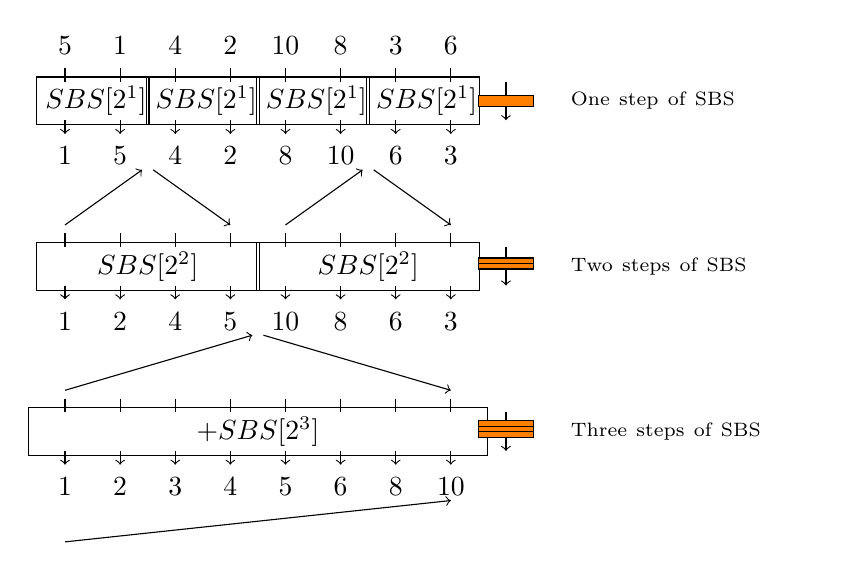
\begin{tikzpicture}[scale=0.7]
    \foreach \x / \it in {5/0,1/1,4/2,2/3,10/4,8/5,3/6,6/7}
    \draw (\it,1) node{\x};
    \foreach \x  in {0,...,7}
    \draw (\x,0.6) -- (\x,0.35);
    \foreach \x / \sg in {0.5/+,2.5/-,4.5/+,6.5/-}
    \draw (\x,0) node[draw,text width=12mm,text centered]{$SBS[2^{1}]$};
    \foreach \x  in {0,...,7}
    \draw[->] (\x,-0.35) -- (\x,-0.6);
    \foreach \x / \it in {1/0,5/1,4/2,2/3,8/4,10/5,6/6,3/7}
    \draw (\it,-1) node{\x};
    %
    \draw[->] (8,0.35) -- (8,-0.35);
    \draw[fill=orange] (7.5,0.1) rectangle (8.5,-0.1);
    \draw (9,0) node[right,text width=3cm]{\scriptsize One step of SBS};
    %
    \draw[->] (0,-2.25) -- (1.4,-1.25);
    \draw[->] (1.6,-1.25) -- (3.,-2.25);
    \draw[->] (4,-2.25) -- (5.4,-1.25);
    \draw[->] (5.6,-1.25) -- (7.,-2.25);
    %
    \foreach \x  in {0,...,7}
    \draw (\x,-2.4) -- (\x,-2.65);
    \foreach \x / \sg in {1.5/+,5.5/-}
    \draw (\x,-3) node[draw,text width=26mm,text centered]{$SBS[2^{2}]$};
    \foreach \x  in {0,...,7}
    \draw[->] (\x,-3.35) -- (\x,-3.6);
    \foreach \x / \it in {1/0,2/1,4/2,5/3,10/4,8/5,6/6,3/7}
    \draw (\it,-4) node{\x};
    %
    \draw[->] (8,-2.65) -- (8,-3.35);
    \draw[fill=orange] (7.5,-2.85) rectangle (8.5,-2.95) rectangle (7.5,-3.05);
    \draw (9,-3) node[right,text width=3cm]{\scriptsize Two steps of SBS};
    %
    \draw[->] (0,-5.25) -- (3.4,-4.25);
    \draw[->] (3.6,-4.25) -- (7.,-5.25);
    \foreach \x  in {0,...,7}
    \draw (\x,-5.4) -- (\x,-5.65);
    \draw (3.5,-6) node[draw, text width=56mm,text centered]{$+SBS[2^{3}]$};
    \foreach \x  in {0,...,7}
    \draw[->] (\x,-6.35) -- (\x,-6.6);
    \foreach \x / \it in {1/0,2/1,3/2,4/3,5/4,6/5,8/6,10/7}
    \draw (\it,-7) node{\x};
    %
    \draw[->] (8,-5.65) -- (8,-6.35);
    \draw[fill=orange] (7.5,-5.8) rectangle (8.5,-5.9) rectangle (7.5,-6.0) rectangle (8.5,-6.1);
    \draw (9,-6) node[right,text width=3cm]{\scriptsize Three steps of SBS};
    %
    \draw[->] (0,-8) -- (7,-7.25);
    \end{tikzpicture}
    
    \end{frame}
    
    \begin{frame}{Bitonic sort analysis}
    
    \alert{Complexity of bitonic sort} :
    \begin{itemize}
    \item With $n=2^{k}$, there are $k$ phases, each involving $1,2,\ldots, k$ steps,
      respectively;
    \item The total number of steps is 
    \begin{equation}
    \sum_{i=1}^{k}i = \frac{k(k+1)}{2} = O(k^{2}) = O(\log_{2}^{2} n)
    \end{equation}
    \item Total complexity is $O(n\log_{2}^{2} n)$
    \end{itemize}
    \end{frame}

    \begin{frame}{Adapt bitonic sort to distributed parallel architecture}
        \scriptsize
        \begin{block}{Main ideas}
            \begin{itemize}
                \item First sort with the fastest sort algorithm local data in increasing values if rank is even and decreasing values if rank is odd;
                \item Pairing inside a subcommunicator  processes to define a bitonic sequence;
                \item And apply bitonic sort algorithm, grouping processes per four, height and so\ldots
                \item Sub-communicators build here are very similar to the sub-communicators build with hyperquick sort algorithms !
            \end{itemize}
        \end{block}

    \end{frame}

\section{Bucket-sort algorithms}
\end{document}
